\documentclass[../../main.tex]{subfiles}

\begin{document}

\chapter{Generator Training} \label{chapter:generatorTraining}

\section{Distribution matching} \label{section:distributionMatching}

\subsection{KL-divergence} \label{subsection:klDivergence}

Because using ANNs requires a space similarity problem to be framed as a distribution similarity problem (\S\ref{section:modellingSpacesAsDistributions}), distribution distance metrics can be used.
If $g'$ is modelled by a network whose p.d.f. can quickly be found, the KL-divergence between $\hat{V_c}'$ and $\hat{V_c}$ can be estimated by drawing samples from $\hat{V'_c}$.
The p.d.f. of an ANN can be found by inverting it or using a constrained architecture such as a radial basis function \cite{park91}.
Whether or not inverting a network is plausible is discussed in \S\ref{section:neuralNetworkInversion}.
The integral form of the KL-divergence is:
\begin{equation}
    D_{\text{KL}}(\hat{V'_c}\;||\;\hat{V_c})=\int_L\hat{V'_c}(g'(l,c))\;\text{log}\bigg(\frac{\hat{V'_c}(g'(l,c))}{\hat{V_c}(g'(l,c))}\bigg)\;\mathrm{d}l
\end{equation}
Since integration over the entirety of the latent space is unlikely to be tractable, this equation can be adapted such that the divergence is written as an expectation across a batch of samples, each weighted by their probability of occurring.
Let $\{l_1,l_2,...,l_{j-1},l_j\}$ be a batch of samples drawn from the latent space.
An estimation of the KL-divergence can then be calculated:
\begin{equation}
    \textbf{E}\big[D_{\text{KL}}(\hat{V'_c}\;||\;\hat{V_c})\big]=\frac{1}{j}\sum_{i=1}^{j}\text{log}\bigg(\frac{\hat{V'_c}(g'(l_i,c))}{\hat{V_c}(g'(l_i,c))}\bigg)
\end{equation}
The term before the logarithm disappears in the summation equation because each sample is weighted by the inverse of its probability density under $\hat{V'_c}$.

Since all operations in this equation are differentiable, the partial derivative of the KL-divergence with respect to the weights of the generator can be found by a library with automatic differentiation such a Tensorflow.
Then $g'$ training is simply a matter of minimising $D_\text{KL}$.

\subsection{Potential issues} \label{subsection:potentialIssues}

While theoretically very simple, there are several practical problems that could arise during training with this approach.
\begin{itemize}
    \item[] \textbf{Exploding gradients}: a problem frequently encountered when minimising functions containing a logarithm is the occurrence of NaN values resulting from taking the logarithm of zero \cite{bengio94}.
    While this will not be an issue since the numerator of the fraction will be non-zero by virtue of the fact that that point has been sampled, very small values are possible.
    Zeros in the denominator are also possible.
    These will produce large negative logarithms, whose derivatives may cause exploding gradients.
    Because it is known that large positive gradients are likely to result from a logarithm, but large negative ones are impossible, it may be possible to clip the derivatives to prevent exploding gradients while still obtaining correct results.   
    \item[] \textbf{Disjoint manifolds}: the points comprising real data distributions are often described in a much higher-dimensional space than the intrinsic dimension of the distribution that created them.
    This will likely be the case for $h$, and so when $g'$ is first initialised it is highly likely that $\hat{V'_c}$ and $\hat{V_c}$ will be disjoint (\S\ref{subsection:pretrainingResults}).
    If this is the case then the KL-divergence will always be 0 and no training will occur.
    Methods of solving this problem, such as minimising the Wasserstein distance instead of KL-divergence, were considered but judged to be beyond the scope of this project.
\end{itemize}

\section{Metric proxies} \label{section:metricProxies}

As discussed in \S\ref{section:modellingSpacesAsDistributions}, modelling spaces as distributions invalidates the equations for $p$ and $r$ that were discussed in \S\ref{section:solutionAndConstraintSpaces}.
Proxy metrics will now be defined for $p$ and $r$, which are intuitively similar to the concepts described for spaces but applicable to distributions.

\subsection{Precision} \label{subsection:precision}

Optimising precision is intended to ensure that as many elements from $V'_c$ as possible are also in $V_c$.
When these are viewed instead as distributions, $\hat{V'_c}$ will likey cover almost the entirety of $S$ but with differing densities.

An adequate precision proxy $\hat{p}(g')$ is one which heavily penalises samples from $\hat{V'_c}$ which are in low-density regions of $\hat{V_c}$.
Infrequently drawn samples from $\hat{V'_c}$ may have high penalties, but these will not have a large impact on the overall precision proxy because they will be outnumbered by more probable samples with low penalties.

Letting $\{l_1,l_2,...,l_{j-1},l_j\}$ be a batch of samples drawn from $L$, the precision proxy can be defined as:
\begin{equation}
    \textbf{E}\big[\hat{p}(g')\big]=-\frac{1}{j}\sum_{i=1}^{j}\text{log}\big(1-h(c,g'(l,c))+\epsilon\big)
\end{equation}
Note that $h(c,s)$ is proportional to $\hat{V_c}$ but is a probability instead of a p.d.f. and so will always be between 0 and 1.

Intuitively, this is equivalent to taking a batch of points from $L$, mapping them into $S$, calculating $h$ for each point, and taking the mean of the negative logarithm of $1$ minus each of these values.
Solutions for which $\hat{V_c}(s)\ll\hat{V'_c}(s)$ will occur frequently (because their density in $\hat{V'}(c)$ is high) but be severely penalised (because $h(c,s)$ is small and so $\text{log}(1-h(c,s))$ will be large).
The result of this is that $g'$ will learn weights that avoid this situation as much as possible.

\subsection{Recall} \label{subsection:recall}

In many ways, recall is the opposite of the precision.
Solutions which are highly likely to satisfy the constraint, but which occur very infrequently in $\hat{V'_c}$, will be penalised.
\begin{equation}
    \textbf{E}\big[\hat{r}(g')\big]=-\frac{1}{j}\sum_{i=1}^{j}\text{log}\big(1-g'^{-1}(s,c)+\epsilon\big)
\end{equation}
where $\{s_1,s_2,...,s_{j-1},s_j\}$ is a batch of solutions drawn from $\hat{V_c}$.
Such a batch can be produced using a Markov chain Monte Carlo method such as the Metropolis-Hastings algorithm \cite{robert16}.
Like direct minimisation of the KL-divergence, $\hat{r}$ assumes that $g'^{-1}$ is tractable.

\subsection{Spread} \label{subsection:spread}

Optimisation for $\hat{p}$ is dependent on high-density regions of $\hat{V_c}$ being sampled at least occasionally by $\hat{V'_c}$, and so it stands to reason that convergence will occur slowly if $\hat{V'_c}(s)\approx 0$ for most $s$.

Training might therefore be accelerated if $g'$ can be pretrained such that it samples from a wide range of $S$ at least sometimes, allowing the highest density regions of $\hat{V_c}$ to be quickly identified.
Some metrics are proposed below which, when minimised, discourage $g'$ from sampling only a small subset of $S$.
\begin{itemize}
    \item[] \textbf{Similarity loss}: penalises according to the squared distance between a point in $L$ and its accompanying point in $S$, when both spaces are linearly scaled such that they are unit hypercubes.
    This effectively forces $g'$ to model the identity function after its initialisation.
    \begin{equation}
        q_\text{id}(g,l,c)=\bigg|\frac{l-a_L}{b_L-a_L}-\frac{g(l,c)-a_S}{b_S-a_S}\bigg|^2
    \end{equation}
    Since any point in $L$ can be sampled, if $g'$ closely approximates the identity function then all points in $S$ will be roughly equally likely to be sampled.
    One clear drawback, however, is that this spread metric requires $m=k$, which may not be desirable for large $m$.
    \item[] \textbf{Separation loss}: a more weakly defined spread metric for use when $m\neq k$.
    Intuitively, it is equivalent to forcing the mean distance between points in $\hat{V'_c}$ towards $q_\text{target}$. 
    \begin{equation}
        q_\text{sep}=\bigg(q_\text{target}-\frac{1}{b^2}\sum_{i,j=1}^b\big|B_i-B_j\big|^2\bigg)^2
    \end{equation}
    where $B=\{B_1,...,B_b\}$ is a batch sampled from $\hat{V'_c}$.
    This spread metric will typically be quite slow because its calculation is of the order $\text{O}(b^2)$ as opposed to the $\text{O}(b)$ for $q_\text{id}$.
\end{itemize}
As well as being used in pretraining for efficient generator initialisation, these spread metrics could be used as a weak substitute for $\hat{r}$ in the event that evaluating $\hat{V'_c}$ is intractable.
While not strictly measuring $\hat{r}$, they prevent $g'$ from only choosing a single point repetitively.

\section{Neural network inversion} \label{section:neuralNetworkInversion}

Some of the proposed training metrics depend on evaluating $\hat{V'_c}$ at a particular point in $S$.
If $g'$ is modelled by an ANN, this is not an obviously tractable problem; this section will explore methods of solving it.

By viewing $g'$ as a series of transforms applied to $\hat{L}$, which is known to be uniform, the space of points which produce a desired output $-$ referred to as the relevant space $R$ $-$ can be backpropagated through each transform.
Integrating over $R$ in $\hat{L}$ will yield the probability density of the desired output.

An ANN is made up of a series of layers, each of which applies three transforms to its input:
\begin{equation}
    y=\sigma(Wx+b)
\end{equation}
where $y$ is the layer output, $x$ is the layer input, $\sigma$ is the activation function, $W$ is the weight matrix, and $b$ is the bias vector.
Depending on the number of rows in $W$, the layer will expand, reduce, or maintain the dimension of the input.
The input dimension is $n_i$ and the output dimension is $n_o$.

\subsection{Bias addition} \label{subsection:biasAddition}

The input which will produce a specific output after the addition of a bias can be found trivially by subtracting the bias vector from the desired output.
\begin{equation}
    y=x+b\implies x=y-b
\end{equation}
As such, the space of relevant inputs is equivalent to the space of relevant outputs translated by $-b$.

\subsection{Square weight multiplication} \label{subsection:squareWeightMultiplication}

A layer in which $W$ is a square matrix has $n_i=n_o$.
There exists exactly one input which produces the desired output assuming that the output is not a null vector and $|W|\neq 0$; both these are generally valid assumptions.
Therefore $R_\text{in}$ can be found by rotating $R_\text{out}$ according to $W^{-1}$.

In general, evaluating $W^{-1}$ computationally expensive, especially when $n_i$ is large.
One special case in which this is not true is when the $W^{-1}=W^T$, which is much more efficient to evaluate, and occurs when $W$ is orthogonal (pure rotation).
Ensuring that $W$ is always orthogonal is discussed in Appendix \ref{appendix:parameterisingOrthogonalMatrices}.

\subsection{Expansive weight multiplication} \label{subsection:expansiveWeightMultiplication}

When $n_o>n_i$, the input is overdefined by the output, hence not every output will have an input which creates it.
An alternate way of looking at this is that the input is fully defined by the first $n_i$ dimensions of the output.
The latter $n_o-n_i$ dimensions of the output are therefore redundant when it comes to producing $R_\text{in}$ from $R_\text{out}$.

The $W$ is therefore constrained such that it is constructed by concatenating a $n_i\times n_i$ orthogonal matrix $W_\text{orth}$ with a $n_o-n_i\times n_i$ matrix whose elements can vary freely, $W_\text{free}$ (Figure \ref{fig:expansiveLayer}).
Then to invert a space of relevant points, any constraints on the latter $n_o-n_i$ dimensions can be ignored, while any remaining constraints are rotated by $W_\text{orth}^{-1}$.
\begin{figure}[H]
    \begin{center}
    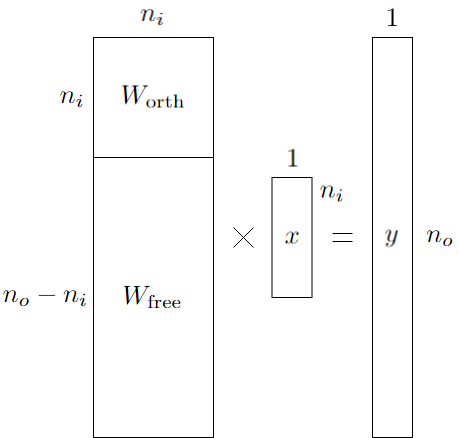
\includegraphics[width=0.45\textwidth]{expansiveLayer}
    \caption{
        Weight matrices which make up an expansive layer in an invertible ANN.
    }
    \label{fig:expansiveLayer}
    \end{center}
\end{figure}

\subsection{Compressive weight multiplication} \label{subsection:compressiveWeightMultiplication}

When $n_o<n_i$ the output underdefines the input.
Generally, the relevant input space is unconstrained and therefore infinite in $n_i-n_o$ dimensions, which is why finding the probability density of a distribution transformed by an ANN requires that each step be able to handle backpropagating relevant spaces as opposed to only points.

Normally, the size of the weight matrix would be $n_o\times n_i$, where $n_i>n_o$.
In this case, however, the weight matrix will be an orthogonal matrix of size $n_i$.
The output vector is obtained by multiplying $W$ by the input, and then retaining only the first $n_o$ components of the resulting vector.

Consider the intermediate step, after multiplying $W$ by the input but before clipping the vector (Figure \ref{fig:compressiveLayer}).
The space of vectors which produce $y$ when retaining only the first $n_o$ components is constrained such that:
\begin{equation}
    x'_j=y_j\;\forall\;1\le j\le n_o
\end{equation}
where
\begin{equation}
    x'=Wx
\end{equation}
while the latter $n_i-n_o$ dimensions can assume any value.
This creates a space which is infinite in some dimensions, but constrained to a single point in others.
The relevant input space can then be obtained by rotating this intermediate space by $W^T$.

Note that the infinite relevant space can be approximated by a finite polytope which extends in each unconstrained dimension to a suitably large distance from the origin, under the reasonable assumption that the activations of hidden units will never greatly exceed $1$.
Therefore $R_\text{in}$ can be described by a set of simplices, also known as a simplicial complex, since any polytope can be constructed from a finite number of simplices \cite{wildberger12}.
Being able to propagate these simplices backwards through the various transforms described in this section is therefore sufficient to all backpropagation of $R_\text{out}$, and thereby find its probability density.
\begin{figure}[H]
    \begin{center}
    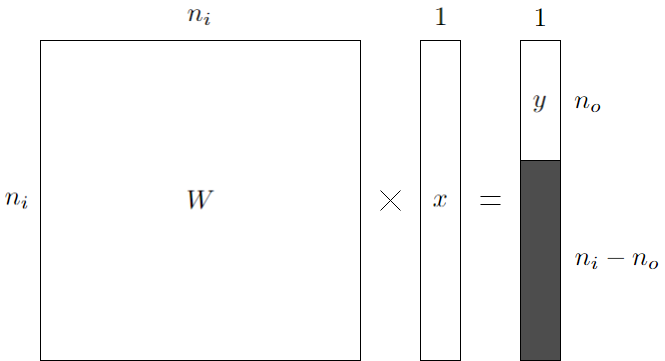
\includegraphics[width=0.7\textwidth]{compressiveLayer}
    \caption{
        Weight matrices which make up a compressive layer in an invertible ANN.
    }
    \label{fig:compressiveLayer}
    \end{center}
\end{figure}

\subsection{Activation} \label{subsection:activation}

Several activation functions are commonly used in ANNs, but here only the ReLU activation function \cite{agarap19} will be considered.
It consists of two linear segments and is applied elementwise to a vector at the end of each layer.

Because the activation function is applied elementwise, the way in which $R_\text{out}$ propagates backwards through a ReLU unit can be considered in terms of each dimension independently.
The following rules can be applied to each dimension:
\begin{enumerate}
    \item any region which is above $0$ can propagate backwards unchanged, since the ReLU function mimics the identity function above $0$;
    \item any region which is below $0$ can be ignored, since the ReLU function will never produce an input which is below $0$;
    \item if $0$ is a possible value in a dimension, all negative values must be added to $R_\text{in}$ in that dimension.
    This is because any negative value in that dimension would have produced an output of $0$.
    Again, simplices extending suitably far from the origin can be used to approximate an extension to infinity.
\end{enumerate}

\subsection{Obstacles} \label{subsection:obstacles}

While theoretically sound, propagating a relevant space backwards through an ANN in order to compute its p.d.f. like thisis not practical.

Problems arise because compressive layers require that a space be propagated back rather than a point.
A simplicial complex can be used to describe this space, but inverting a simplicial complex through a ReLU activation function is impractical for two reasons.

The first is that inverting each simplex requires determining how it intersects with an axis, if at all.
While algorithms exist for doing this in three dimensions or fewer, it appears that an algorithm for $n$ dimensions does not yet exist \cite{wildberger12}.

Secondly, the inversion requires that each simplex splits in two upon meeting the zero of an axis.
If it intersects with the zeros of $i$ axes simultaneously, it must be split into $2^i$ different simplices.
While this split will not occur every time a simplex is propagated back through a ReLU activation, the potential for such an exponential growth could quickly become unmanageable.

Other activation functions which do not consist of linear segments will suffer even greater problems since a simplex is a fundamentally linear shape.

For this reason, methods which require the evaluation of the p.d.f. of an ANN will not be pursued further in this project.

\section{Training procedure} \label{section:generatorTrainingProcedure}

This section assumes that $h$ is either already known, or approximated by $h'$.
That process is explored in greater depth in the \S\ref{chapter:discriminator}.

Training broadly consists of two steps: pretraining, which involves initialising $g'$ to explore a reasonable subset of $S$; and training, in which $g'$ is trained to balance $\hat{p}$ and $\hat{r}$.

\subsection{Pretraining} \label{subsection:pretraining}

A batch of samples are taken from $\hat{L}$ and passed through $g'$ into $S$.
Unless otherwise required by the environment, constraints can also be sampled uniformly from $C$.
Using these values, the spread loss of $g'$ is calculated according to either $q_\text{id}$ or $q_\text{sep}$, whichever is deemed more appropriate.

In the backward pass, the partial derivative of $q$ is calculated with respect to each generator parameter.
Gradients are applied using a gradient descent algorithm such as Adam \cite{kingma17}.

This process is repeated until either the parameters converge or $q$ is sufficiently low.

\subsection{Training} \label{subsection:training}

In the main training phase, latent points are sampled uniformly and constraints are sampled as in the pretraining phase.
They are matched into arbitrary pairs, each one comprising a data point.
The constraint vector is fed to both $h'$ and embedder (which in turn feeds its values to the last layer of $g'$), while $l$ is fed to $g'$.

From these inputs, $s$ is calculated, and the likelihood of its satisfying $c$ is calculated from $h'$.
Given all these values, $\hat{p}$ and $\hat{r}$ (or one of $q_\text{id},q_\text{sep}$ in place of $\hat{r}$) can be calculated and combined into a weighted loss term.
Again, the derivatives of this value are used to minimise the weights of $g'$.
If $h'$ is an ANN, its weights remain fixed throughout this process.

\end{document}
